\documentclass[12pt, letterpaper, twoside]{article}
\usepackage{nopageno,epsfig, amsmath, amssymb}
\usepackage{physics}
\usepackage{mathtools}
\usepackage{hyperref}
\usepackage{xcolor}
\usepackage{mhchem}
\hypersetup{
    colorlinks,
    linkcolor={blue},
    citecolor={blue},
    urlcolor={blue}
}
\usepackage{empheq}
\usepackage{wrapfig}

\usepackage[letterpaper,
            margin=0.8in]{geometry}

\newcommand{\psetnum}{3}
\newcommand{\class}{ASTR 531 - Stellar Interiors and Evolution}

\newcommand{\tomtitle}{
    \noindent {\LARGE \fontfamily{cmr}\selectfont \textbf{\class}} \hfill \\[1\baselineskip]
    \noindent {\large \fontfamily{cmr}\selectfont Problem Set \psetnum \hfill \textsc{Tom Wagg}}\\[0.5\baselineskip]
    {\fontfamily{cmr}\selectfont \textit{\today}}\\[2\baselineskip]
}

\title{\class : Problem Set \psetnum}
\author{\textbf{Tom Wagg}}

\newcommand{\question}[1]{{\noindent \it #1}}
\newcommand{\answer}[1]{
    \par\noindent\rule{\textwidth}{0.4pt}#1\vspace{0.5cm}
}
\newcommand{\todo}[1]{{\color{red}\begin{center}TODO: #1\end{center}}}

% custom function for adding units
\makeatletter
\newcommand{\unit}[1]{%
    \,\mathrm{#1}\checknextarg}
\newcommand{\checknextarg}{\@ifnextchar\bgroup{\gobblenextarg}{}}
\newcommand{\gobblenextarg}[1]{\,\mathrm{#1}\@ifnextchar\bgroup{\gobblenextarg}{}}
\makeatother

\newcommand{\avg}[1]{\left\langle #1 \right\rangle}
\newcommand{\angstrom}{\mbox{\normalfont\AA}}
\allowdisplaybreaks

\begin{document}

\tomtitle

\question{\textbf{12.2 - Early Radii and Timescales}}

\question{Part a - Radii Estimations}
\answer{
    Let's use a couple of different relations from the textbook to get the radii at different times. A protostar becomes ionised and stars the Hayashi concentration phase when it's radius is on the order of (Eq. 12.13)
    \begin{equation}
        R_{\rm Hayashi, start} \approx 100 \unit{R_{\odot}} \qty(\frac{M}{\unit{M_\odot}})
    \end{equation}
    We find the radius of the protostar once the Hayashi concentration phase comes to an end is approximately a factor of 50 lower (based on assumptions of the temperature and opacity) such that (page 12-8)
    \begin{equation}
        R_{\rm Hayashi, end} \approx 2 \unit{R_{\odot}} \qty(\frac{M}{\unit{M_\odot}})
    \end{equation}
    The radius at the start of the PMS phase is the same as the end of the Hayashi concentration phase.
    \begin{equation}
        R_{\rm PMS, start} = R_{\rm Hayashi, end}
    \end{equation}
    Finally, the radius at the end of the PMS phase is the same as the radius at ZAMS and so we can write that (Eq. 12.16)
    \begin{equation}
        R_{\rm PMS, end} = R_{\rm ZAMS} = \unit{R_\odot} \qty(\frac{M}{\unit{M_\odot}})^{0.7}
    \end{equation}
    So now we can plug in numbers for the different masses of stars that we considered
    \begin{center}
        \begin{tabular}{c|cccc}
            $M / \unit{M_\odot}$ & $R_{\rm Hayashi, start} / \unit{R_\odot}$ & $R_{\rm Hayashi, end} / \unit{R_\odot}$ & $R_{\rm PMS, start} / \unit{R_\odot}$ & $R_{\rm PMS, end} / \unit{R_\odot}$ \\
            \hline
            0.3 & 30 & 0.6 & 0.6 & 0.43 \\
            3 & 300 & 6 & 6 & 2.16 \\
            30 & 3000 & 60 & 60 & 10.8 \\
        \end{tabular}
    \end{center}
}

\question{Part b - Timescale estimations}
\answer{
    The duration of the Hayashi concentration phase is given in Eq. 12.15 but we also showed that the timescale scales as $1 / M$ such that
    \begin{equation}
        \tau_{\rm Hayashi} \approx 10^{6} \unit{yr} \qty(\frac{M_{\odot}}{M})
    \end{equation}
    The duration of the PMS phase is given by Eq. 12.17 so we have that
    \begin{equation}
        \tau_{\rm PMS} \approx 6 \times 10^7 \unit{yr} \qty(\frac{M}{\unit{M_\odot}})^{-2.5}
    \end{equation}
    So now we can plug in numbers for the different masses of stars that we considered
    \begin{center}
        \begin{tabular}{c|cc}
            $M / \unit{M_\odot}$ & $\tau_{\rm Hayashi} / \unit{yr}$ & $\tau_{\rm PMS} / \unit{yr}$ \\
            \hline
            0.3 & $3.33 \times 10^6$ & $1.22 \times 10^9$ \\
            3 & $3.33 \times 10^5$ & $3.85 \times 10^6$ \\
            30 & $3.33 \times 10^4$ & $1.22 \times 10^4$ \\
        \end{tabular}
    \end{center}
}

\question{\textbf{15.4 - Metallicity and Mass Loss Rates}}
\answer{
    I found it easier to grab the files from online rather than copy them from the textbook so it was easy enough to just do this for all of the masses rather than only $20 \unit{M_\odot}$ and $60 \unit{M_\odot}$.

    You can see how I calculated the mass loss rates in \href{https://github.com/TomWagg/uw-grad-classes/blob/main/531_stars/pset3/code.ipynb}{this Jupyter notebook} using Vink (2001) mass loss (Eq.\ 15.14). The exact values at ZAMS and TAMS are under ``Part a Answers'' if you want to see them. I'm going to brush over those because they're just numbers and instead focus on the later parts which are easier to qualitatively discuss.

    In the plots below I show the average MS mass loss rate (averaged between ZAMS and TAMS) on the left, and I then multiply this by the length of the main sequence to get the fraction of mass that is lost, shown on the right. The dotted lines show the `real' mass loss rate which was contained in the files. We can see that the rates I calculated match up rather well with these!
    \begin{center}
        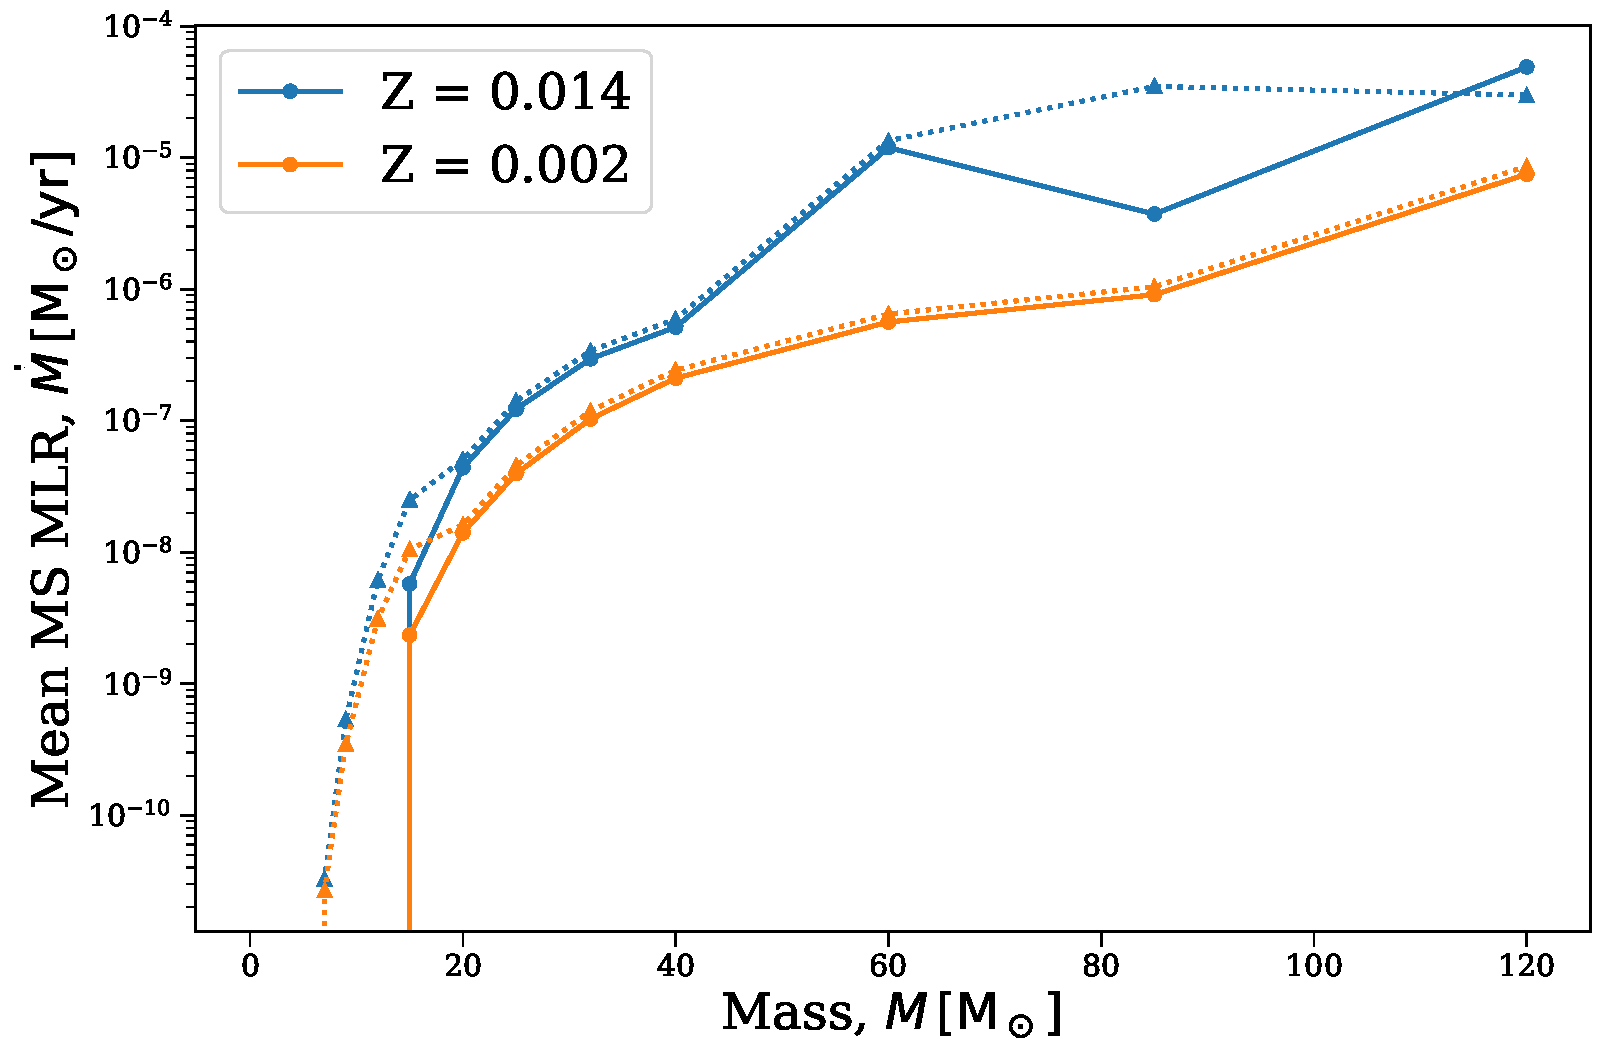
\includegraphics[width=0.495\textwidth]{figures/mean_MS_mlr.pdf}
        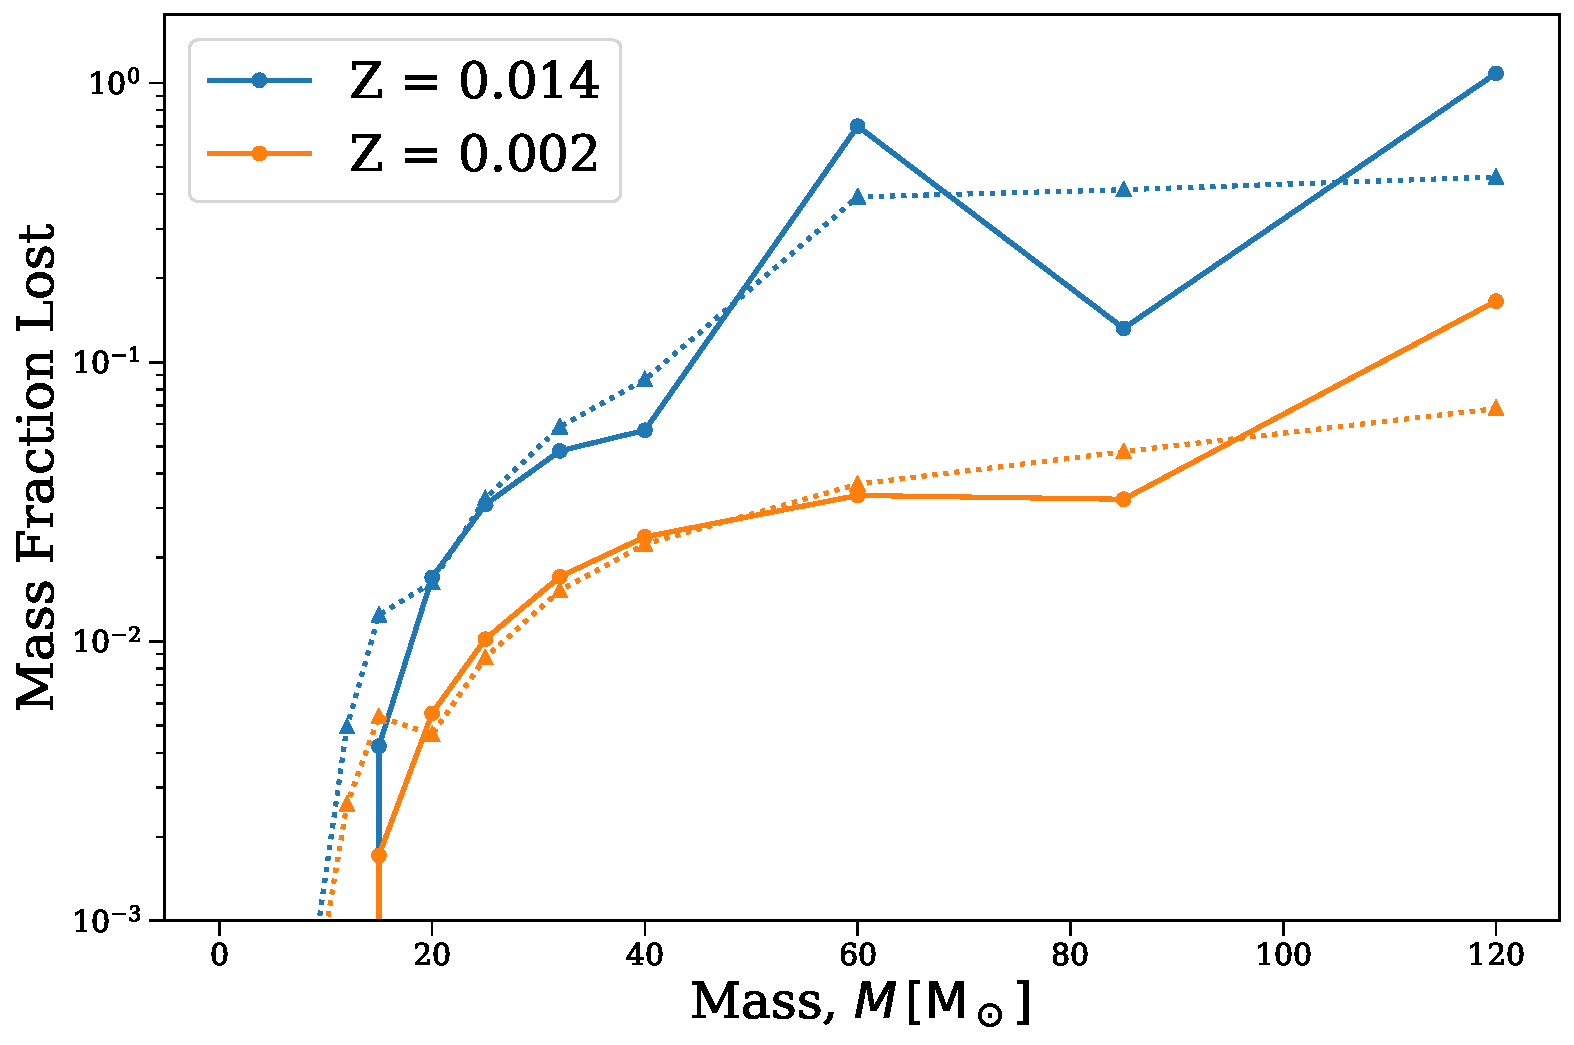
\includegraphics[width=0.495\textwidth]{figures/mass_fraction_lost.pdf}
    \end{center}
    \textbf{Metallicity Effects:} First, let's talk about what happens for the different metallicities. You can immediately see that the higher metallicity line (blue) is much higher than the low metallicity line (orange) - note these are log scales! The lower metallicity stars have fewer metals and thus fewer lines that can be used to drive winds. Therefore mass loss is lower for lower metallicity stars.

    \noindent We also see that my calculated rates don't quite match up with those in the files so let's just address that quickly. First the overall rates seem to be lower pretty much everywhere. This makes sense because we are only calculating one type of winds but the files include lots of different winds.
    
    \textbf{Small mass differences:} For masses below $20 \unit{M_\odot}$ we seem to be under-predicting the mass loss rates and this makes sense because Vink mass loss only applies to hot and luminous stars and are zero for these stars (specifically for anything with $T_{\rm eff} < 12500 \unit{K}$ or $L < 3 \times 10^4 \unit{L_\odot}$). If we added the Nieuwenhujzen \& de Jager fit then those winds would probably explains most of the difference (since these are just main sequence stars.)
    
    \textbf{Large mass differences:} For masses above $80 \unit{M_\odot}$ things start to go wrong as well. For an $85 \unit{M_\odot}$ star, we are under-predicting the mass loss by nearly an order of magnitude. I \textit{think} this might be LBV winds in the real model. I'm honestly unsure why we over-predict for a $120 \unit{M_\odot}$ but the Vink fits aren't supposed to be used above 50,000 K anyway so we're in dodgy regions anyway. If there's an obvious reason for this I'd love to know! :)
}

\question{\textbf{16.1 - RGB Radii}}
\answer{
    From inspection of Figure 16.1 we can find values for $L$ and $T_{\rm eff}$ at the start and end of the RGB phase. This phase starts at C and ends at F. We can then use the fact that
    \begin{equation}
        R = \sqrt{\frac{L}{4 \pi \sigma T_{\rm eff}^4}}
    \end{equation}
    to get the radii. Since I'm in a mood for tables today, let's make another!
    \begin{center}
        \begin{tabular}{c|ccc}
            Stage & $\log (L / \unit{L_\odot})$ & $\log (T_{\rm eff} / \unit{K})$ & $R / \unit{R_{\odot}}$ \\
            \hline
            C (Start of RGB) & 0.4 & 3.7 & 2.1 \\
            F (End of RGB) & 3.4 & 3.48 & 183.1
        \end{tabular}
    \end{center}
    So the radius is increasing by nearly two orders of magnitude!
}

\question{\textbf{17.1 - Helium Flash Duration}}
\answer{
    First we need to calculate the potential energy of a uniform sphere. We know that gravitational potential is given by
    \begin{equation}
        \Phi = - \frac{G M}{r}
    \end{equation}
    So we just need to integrate this over a series of teeny tiny shells over the core of the star. Note we can assume a uniform density so $\rho(r) = \rho$. Let's do it!
    \begin{align}
        U &= - \int_0^R \frac{G M(r)}{r} \rho(r) \dd[3]{r} \\
          &= - \int_0^R \frac{G (\rho(r) \frac{4}{3} \pi r^3)}{r} \rho(r) 4 \pi r^2 \dd{r} \\
          &= - \frac{16 G \pi^2 \rho^2}{3}\int_0^R r^4 \dd{r} \\
        U &= - \frac{16 G \pi^2 \rho^2 R^5}{15}
    \end{align}
    We can rearrange this to get rid of the radius and just write it as a function of density and mass.
    \begin{align}
        R &= \qty(\frac{3 M}{4 \pi \rho})^{1/3} \\
        U &= - \frac{16 G \pi^2 \rho^2}{15} \qty(\frac{3 M}{4 \pi \rho})^{5/3} \\
        U &= - \frac{G \qty(36 \pi M^5 \rho)^{1/3}}{5}
    \end{align}
    Nice, what a...clean expression?\footnote{To be fair, it looks much better if we did it in terms of $M$ and $R$: $U = -\frac{3}{5} G M^2 / R$}. Now let's use this to find the difference in potential energy for a $0.5 \unit{M_\odot}$ core expanding from a density of $\rho = 10^{6} \unit{g}{cm^{-3}}$ to $\rho = 10^{4} \unit{g}{cm^{-3}}$.
    \begin{equation}
        \Delta U = - \frac{G \qty(36 \pi (0.5 \unit{M_\odot})^5)^{1/3}}{5} \qty[(10^{4} \unit{g}{cm^{-3}})^{1/3} - (10^{6} \unit{g}{cm^{-3}})^{1/3}] = 5 \times 10^{42} \unit{J}
    \end{equation}
    Now we can calculate the duration of the Helium flash given the energy production and efficiency
    \begin{equation}
        \tau_{\rm flash} = \frac{\Delta U}{L \cdot \phi} = \frac{5 \times 10^{49} \unit{J}}{10^{10} \unit{L_\odot} \cdot 0.2} = 2.5 \times 10^{40} \unit{erg}{L_\odot^{-1}}
    \end{equation}
    Now because I'm an ``astronomer'' I can 100\% (totally) understand ergs and $L_\odot$ intuitively, but just in case some readers don't live and breathe cgs in the same way this translates to
    \begin{equation}
        \boxed{ \tau_{\rm flash} = 0.21 \unit{yr} \approx 76 \unit{days} }
    \end{equation}
    Quite the `flash' indeed!
}

\end{document}

 